% Figure 6, composed: panel (a), the vector cartoon, is drawn here in TikZ into the place that dramatis
% scripts/paper_fig.py leaves empty in figures/fig6_mechanism_base.pdf (its box: figures/fig6_slot.tex).
% Words in Arial, as in the matplotlib panels (hence lualatex); math in Latin Modern, as in the text.
% Built by `make figures`, run from the paper's root: -> figures/fig6_mechanism.pdf
\documentclass[border=0pt]{standalone}
\usepackage{lmodern}
\usepackage[no-math]{fontspec}
\setsansfont{Arial}
\usepackage{amsmath,bm}
\usepackage{tikz}
\usetikzlibrary{arrows.meta,calc}
\pgfdeclarelayer{lines}
\pgfsetlayers{lines,main}  % the lines under the points, so they run from edge to edge
\definecolor{villain}{HTML}{C62828}
\definecolor{kind}{HTML}{1F5FAE}
\definecolor{classvec}{HTML}{6A3D9A}  % the class vector g, and steering by it (paper_fig.py's STEER_C)
\definecolor{muted}{HTML}{898781}
\definecolor{text}{HTML}{333333}  % paper_fig.py's TEXT, the color of its annotations
\input{figures/fig6_slot}
\newsavebox\cartoon
\begin{document}
\sbox\cartoon{%
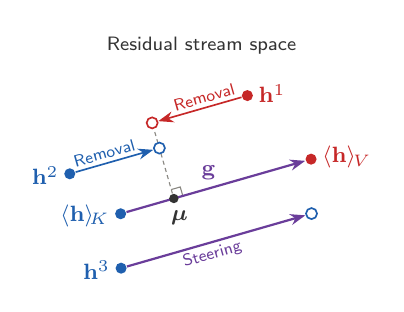
\begin{tikzpicture}[x=0.74cm,y=0.74cm,
    >={Stealth[length=5.5pt,width=4pt]},
    dot/.style={circle,inner sep=0pt,minimum size=4pt,fill=#1},
    ring/.style={circle,inner sep=0pt,minimum size=4pt,draw=#1,fill=white,line width=0.6pt},
    math/.style={font=\footnotesize,text=#1,inner sep=1.5pt},
    word/.style={font=\sffamily\fontsize{6}{7.2}\selectfont,text=#1,transform shape,inner sep=1.5pt}]  % 6 pt, as paper_fig.py's annotations; turned with the scope
  \begin{scope}[rotate=16]
    % the class means and mu on g; a villain and a kind item before (filled) and after (open) removal; a kind name
    % before and after steering. Rows: the kind item and the steered name equally far from g, the villain item
    % 1.5 times as far (the two removals read as a pair)
    \pgfmathsetmacro\rowd{0.9}
    \pgfmathsetmacro\rowv{1.5*\rowd}
    \node[dot=kind] (K) at (0,0) {};
    \node[dot=villain] (V) at (3.4,0) {};
    \node[dot=text,minimum size=3.4pt] (M) at (0.95,0) {};
    \node[dot=villain] (Vb) at (2.65,\rowv) {};
    \node[ring=villain] (Vb2) at (0.95,\rowv) {};
    \node[dot=kind] (Kb) at (-0.65,\rowd) {};
    \node[ring=kind] (Kb2) at (0.95,\rowd) {};
    \node[dot=kind] (Kc) at (-0.25,-\rowd) {};
    \node[ring=kind] (Kc2) at (3.15,-\rowd) {};
    \begin{pgfonlayer}{lines}
      % removal: onto the line through mu perpendicular to g
      \draw[muted,dash pattern=on 1.5pt off 1.2pt,line width=0.4pt] (M) -- (Vb2);  % short dashes: two or three between the circles
      \draw[muted,line width=0.4pt] (0.95,0.16) -- (1.11,0.16) -- (1.11,0);  % the right angle at mu
      \draw[->,classvec,line width=0.8pt] (K) -- (V);
      \draw[->,villain,line width=0.6pt] (Vb) -- (Vb2);
      \draw[->,kind,line width=0.6pt] (Kb) -- (Kb2);
      \draw[->,classvec,line width=0.8pt] (Kc) -- (Kc2);  % steering: a kind name moved by the whole of g
    \end{pgfonlayer}
    % the arrows' labels centered on their shafts: the midpoint moved back by half the head (5.5 pt)
    \node[math=classvec,above=1.5pt] at ($($(K)!0.5!(V)$)!2.75pt!(K)$) {$\mathbf g$};
    \node[word=villain,above] at ($($(Vb)!0.5!(Vb2)$)!2.75pt!(Vb)$) {Removal};
    \node[word=kind,above] at ($($(Kb)!0.5!(Kb2)$)!2.75pt!(Kb)$) {Removal};
    \node[word=classvec,below] at ($($(Kc)!0.5!(Kc2)$)!2.75pt!(Kc)$) {Steering};
    \node[math=text] at ($(M)+(0,-7.4pt)$) {$\bm\mu$};  % on the perpendicular, as far from mu as g from its arrow
    % the points' labels outside them, along g (offsets in the scope turn with it), 2.5 pt from the centers
    \node[math=kind,anchor=east] at ($(K)+(-2.5pt,0)$) {$\langle\mathbf h\rangle_{\mkern-3.5mu K}$};
    \node[math=villain,anchor=west] at ($(V)+(2.5pt,0)$) {$\langle\mathbf h\rangle_{\mkern-2mu V}$};
    \node[math=villain,anchor=west] at ($(Vb)+(2.5pt,0)$) {$\mathbf h^1$};
    \node[math=kind,anchor=east] at ($(Kb)+(-2.5pt,0)$) {$\mathbf h^2$};
    \node[math=kind,anchor=east] at ($(Kc)+(-2.5pt,0)$) {$\mathbf h^3$};
  \end{scope}
  % the panel's heading, 7.5 pt as the axis labels, centered over the drawing
  \node[font=\sffamily\fontsize{7.5}{9}\selectfont,text=text,anchor=south] at ([yshift=5pt]current bounding box.north) {Residual stream space};
\end{tikzpicture}}%
\typeout{Figure 6(a): \the\wd\cartoon\space by \the\dimexpr\ht\cartoon+\dp\cartoon\relax, in a \slotw bp by \sloth bp place}%
\begin{tikzpicture}
  \node[anchor=south west,inner sep=0] at (0,0) {\includegraphics{figures/fig6_mechanism_base.pdf}};
  \node[inner sep=0] at ({\slotx bp + 0.5*\slotw bp}, {\sloty bp + 0.5*\sloth bp}) {\usebox\cartoon};  % centered in its place
\end{tikzpicture}
\end{document}
